\subsection{Arquitectura}
En este apartado se explicarán los componentes que forman parte de la arquitectura de la solución, el cómo se deben conectar para emular una red de FL y el propio montaje físico de los dispositivos. De esta forma, se podrá comprender porque se han seleccionado los dispositivos que van a participar en el FL, cuál es el mapa de red de una red de FL, como se va a representar localmente y como queda el montaje de todos los dispositivos acorde al mapa de red.  

\subsubsection{Componentes}
Para la recreación de un ejemplo real de una red de FL se han utilizado dispositivos de capacidad de cómputo acotada como son las Raspberries Pi. De esta forma, se pretende demostrar la viabilidad de la aplicación del FL a campos como el del internet de las cosas, donde los dispositivos participantes disponen de escasa capacidad de cómputo.
\\ \\
De la misma forma, con el objetivo de demostrar que no se necesita un supercomputador para realizar una agregación de modelos, se ha utilizado la NVIDIA Jetson Nano como núcleo central para ello.
\\ \\
Los dispositivos que se utilizarán en concreto son los siguientes: (x4) Raspberry Pi 3 B+ (Fig. \ref{fig:RaspBerrryBPlus}), (x1) NVIDIA Jetson Nano 2GB (Fig. \ref{fig:JetsonNano2GB}) y (x1) Genius switch (Fig. \ref{fig:Switch}).

\begin{figure}[H]
    \begin{minipage}[t]{0.49\linewidth}  % <---
        \centering
        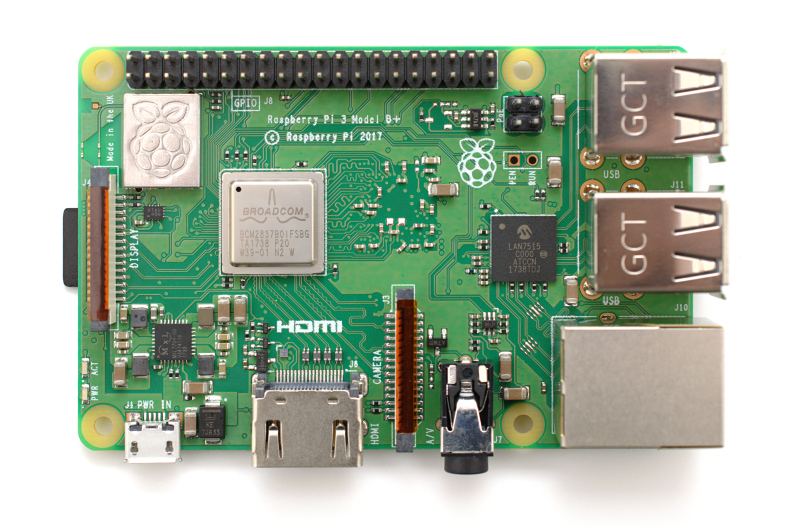
\includegraphics[height=0.1\textheight]{Figuras/Raspberry_Pi_3_B+.png}
        \caption{Raspberry Pi 3 B+ \\ (Fuente: Wikipedia\autocite{ArchivoRaspberryPi})} 
        \label{fig:RaspBerrryBPlus}
    \end{minipage}
    \hfill
    \begin{minipage}[t]{0.5\linewidth}  % <---
        \centering
        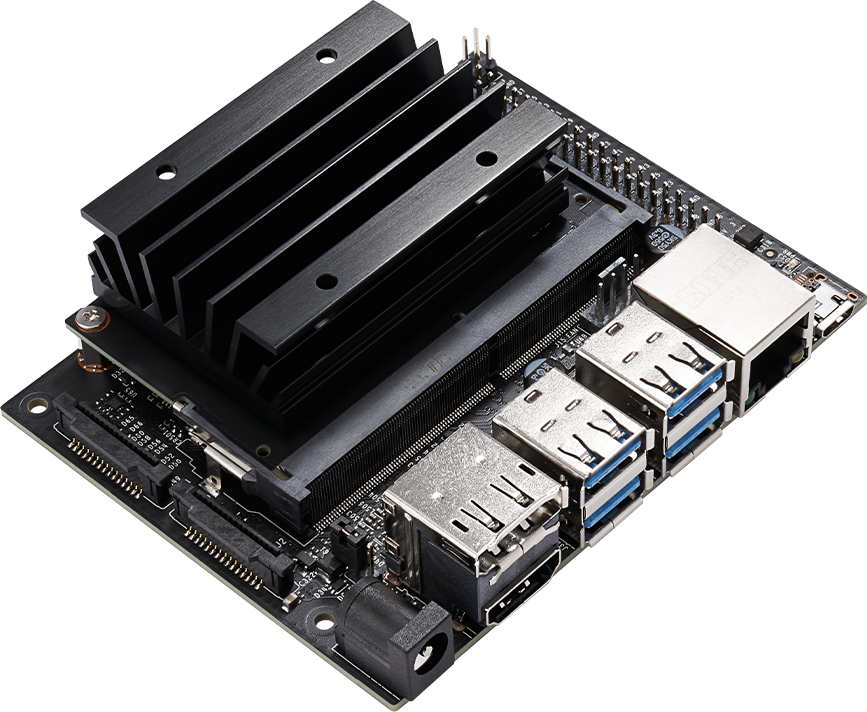
\includegraphics[height=0.1\textheight]{Figuras/nvidia_jetson_nano_2GB.png}    
        \caption{NVIDIA Jetson Nano 2GB \\ (Fuente: NVIDIA\autocite{JetsonNano})} 
        \label{fig:JetsonNano2GB}
    \end{minipage}
\end{figure}
\begin{figure}[H]
    \centering
    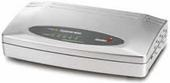
\includegraphics[height=0.1\textheight]{Figuras/genius_switch.jpg}    
    \caption{Switch Genius} 
    \label{fig:Switch}
\end{figure}
\newpage

\subsubsection{Mapa de red}
Las conexiones entre los dispositivos que interactúan en la red (Raspberries y Jetson Nano) será por cable, conectando todos al mismo switch para permitir la comunicación entre ellos. A su vez, este switch se conectará al router que provee de acceso a internet, permitiendo así, que los ordenadores de la red puedan acceder a estos dispositivos y estos dispositivos puedan conectarse a internet para lo que necesiten. Todo ello queda representado en el mapa de de la figura \ref{fig:MapaRed}, que sería el mapa de red físico del que parte el proyecto.
\begin{figure}[H]
    \centering
    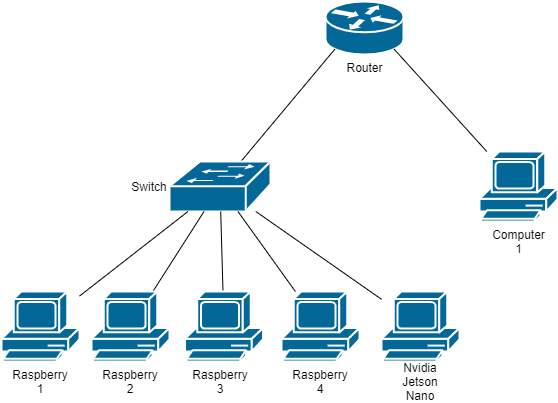
\includegraphics[width=\textwidth]{Figuras/Network_map.png}    
    \caption{Mapa de red física} 
    \label{fig:MapaRed}
\end{figure}

Esta arquitectura de red lo que permite es que desde el ordenador 1 se pueda acceder a cualquier dispositivo mediante ssh para su configuración y ejecución de experimentos. A su vez, estos dispositivos permanecen físicamente separados los unos de los otros mientras mantienen acceso a internet para realizar tareas de descarga de paquetes, actualizaciones, envío de datos, etc. En este caso, para la transferencia de archivos y ficheros se utilizará el protocolo SCP, ya que no entra dentro del alcance el desarrollo de ningún sistema de comunicación y el protocolo SCP es fácilmente combinable con el protocolo ssh.

\pagebreak

Sin embargo, desde el punto de vista de la red de FL que se quiere simular, el mapa de red incluiría los siguientes cambios:
\begin{itemize}
    \item Cada participante tendría su propia red de área local.
    \item La conexión al servidor de agregación se haría a través de internet.
    \item Los participantes no tendrían ninguna conexión ni relación entre sí.
\end{itemize}
De este modo, el mapa de la red de FL representado en el proyecto quedaría acorde a la figura \ref{fig:FLMapaRed}, aunque el mapa de red sobre el que se opere físicamente sea el de la figura \ref{fig:MapaRed}.

\begin{figure}[H]
    \centering
    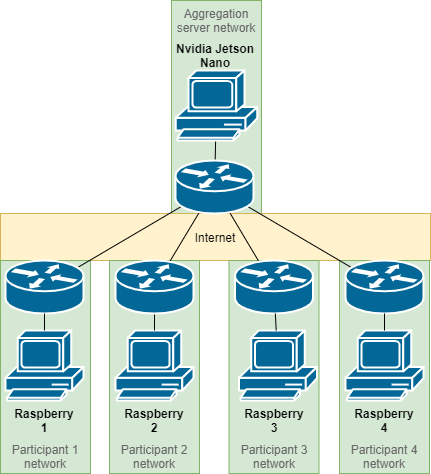
\includegraphics[width=0.8\textwidth]{Figuras/FL_network_map.png}    
    \caption{Mapa de la red de FL} 
    \label{fig:FLMapaRed}
\end{figure}

\pagebreak

\subsubsection{Montaje físico}
Una vez realizados todos los mapas y diagramas para la configuración de la red, se procedió a conectar los dispositivos acorde al mapa de red físico (fig. \ref{fig:MapaRed}). Para este montaje, se acoplaron las Raspberries que representan a los participantes en el rack mencionado en la sección de gestión de riesgos \ref{GestionRiesgos} de este mismo capítulo. Después de conectar todos los cables el montaje quedó como se puede ver en las siguientes imágenes.
\begin{figure}[H]
    \centering
    \begin{minipage}[t]{0.49\linewidth}  % <---
        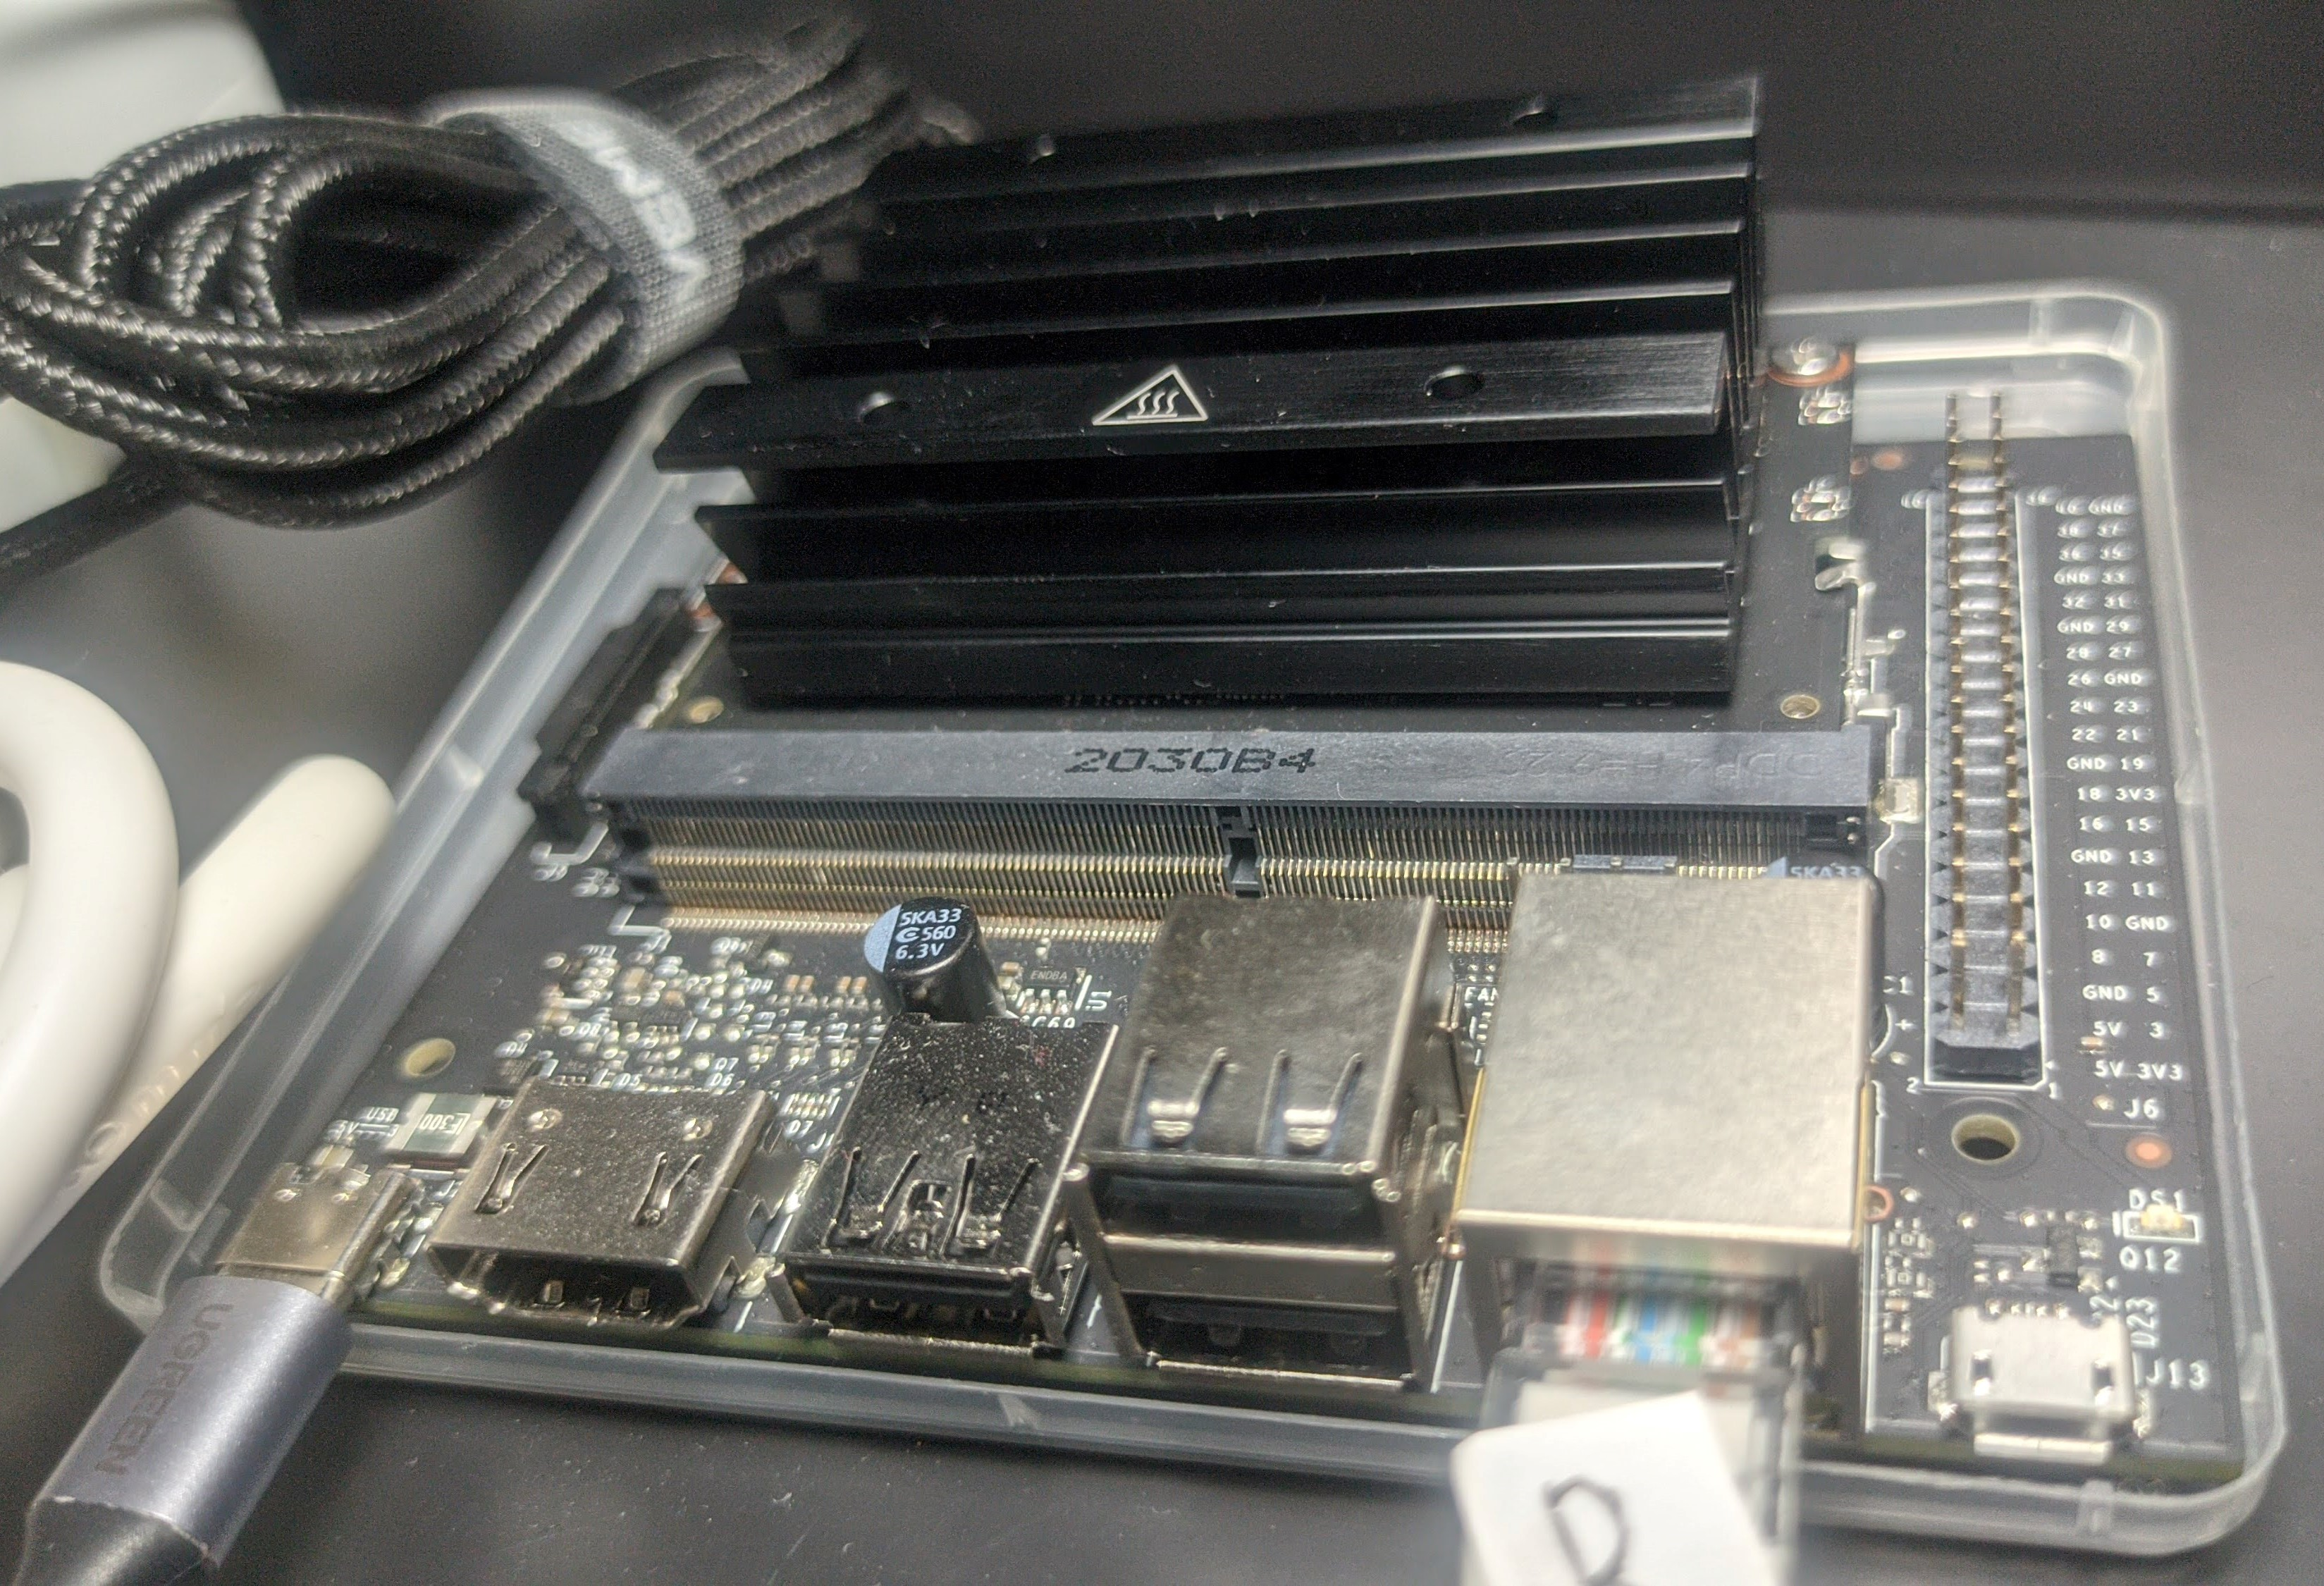
\includegraphics[height=0.2\textheight]{Figuras/jetsonnano.jpg}
        \caption{Montaje de la Jetson Nano} 
    \end{minipage}
    \hfill
    \begin{minipage}[t]{0.5\linewidth}  % <---
        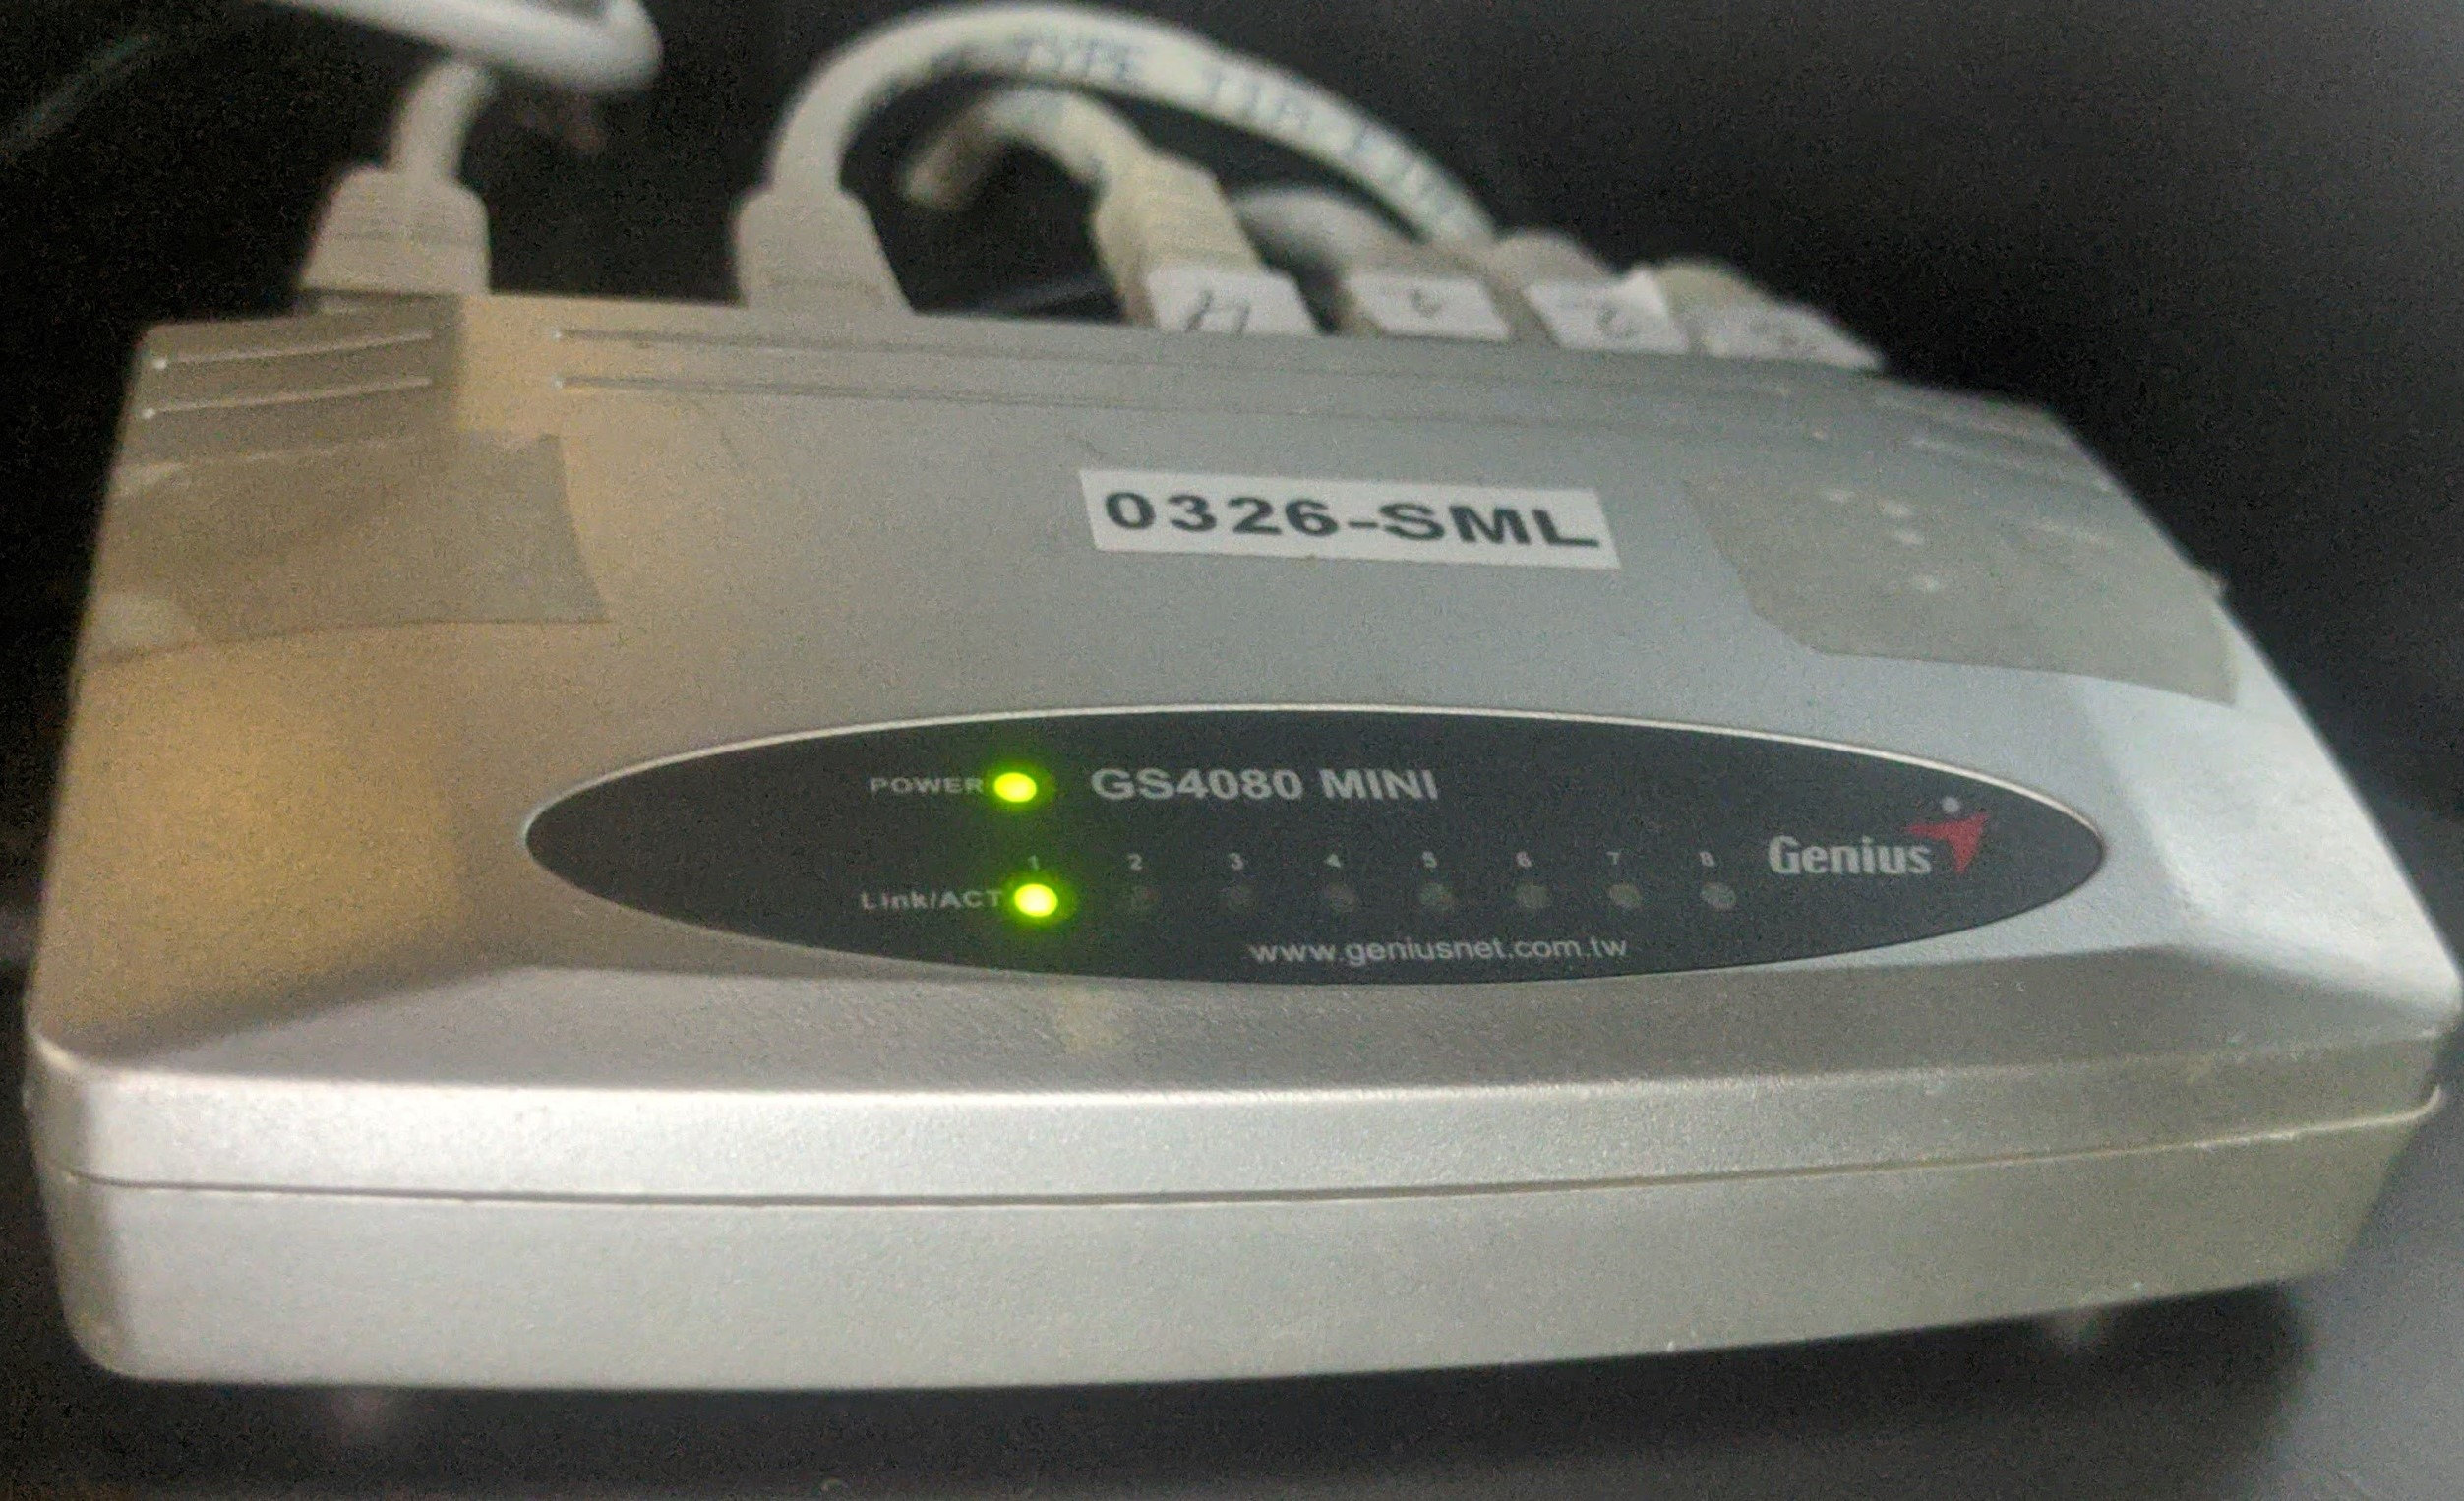
\includegraphics[height=0.2\textheight]{Figuras/switch.jpg}
        \caption{Montaje del switch} 
    \end{minipage}

    \includegraphics[width=0.75\textwidth]{Figuras/raspberrys.jpg}
    \caption{Montaje de las Raspberries}     
\end{figure}

La Jetson Nano y cada Raspberry tienen un cable ethernet conectado al switch, el cual, a su vez, cuenta con otro cable ethernet por el cual se conecta al router (no visible en las fotos).
